\section{Problem Formulation}
\label{sec:problem}

\subsection{Dense-Intelligence Tasks}

The public \systemname formulation defines a \emph{dense-intelligence task} as one that
sustains high-frequency reasoning, tool use, verification, and iteration across a
continuous time window until it produces a measurable result~\citep{argus_site}.
Three conditions determine whether a task has this shape:

\begin{enumerate}[label=\textbf{T\arabic*.}]
  \item \textbf{Invention.} The answer is not directly retrievable from a manual or
    database; it must be discovered through search and feedback.
  \item \textbf{Long horizon.} One pass is insufficient. Progress requires many
    dependent iterations over hours or days.
  \item \textbf{Verifiability.} A task-native evaluator can distinguish genuine
    improvement from a persuasive but incorrect claim.
\end{enumerate}

The defining loop is therefore proposal $\rightarrow$ execution $\rightarrow$
measurement $\rightarrow$ revised proposal. Performance engineering, security
research, scientific search, and quantitative research differ in domain but share
this operational structure. The task definition excludes both open-ended ideation
without an evaluator and fixed workflows that require time but no new decisions.

We model a campaign by an objective $o$, an initial artifact $y_0$, an evaluation
procedure $f$, and a resource budget $B$. The artifact may be code, a model, a
dataset, an experimental harness, a proof, or a manuscript. The campaign is divided
into bounded missions indexed by $t$, each producing

\begin{equation}
  \tau_t=\bigl((s_{t,j},a_{t,j},y_{t,j},e_{t,j},r_{t,j})\bigr)_{j=1}^{n_t},
  \label{eq:trajectory}
\end{equation}

where round $j$ has state $s_{t,j}$, actions $a_{t,j}$, resulting artifact state
$y_{t,j}$, observed measurements $e_{t,j}$, and recorded review or admission outcome
$r_{t,j}$. A mission
must terminate, pause, or transfer control explicitly; continuity belongs to the
persistent campaign state rather than an unbounded model session.

\begin{paperbox}{Report-level contract model}
For analysis, we summarize the working task as
$K_t=(\iota,o_t,c_t,v_t)$: standing intent, current objective, known constraints,
and verification criteria. $X_t$ denotes only the clarifications, priorities, and
unresolved questions made explicit at the user interface. A material refinement is
written compactly as
\[
  (X_{t+1},K_{t+1})
  =\operatorname{ManagerAdmit}(X_t,K_t,K'_t,e_t,r_t,u_t),
\]
where $K'_t$ is the proposed contract, $e_t$ is evidence, $r_t$ the recorded
admission outcome, and $u_t$ the authorized operator or Manager
decision. \code{ManagerAdmit} is a normative operator, not one atomic production
API: it projects over current \code{GoalContract} revisions, persisted operator
questions, Planner replanning, Manager Stage/routing transitions, and append-only
provenance.
\end{paperbox}

Figure~\ref{fig:horizon-mountain} contrasts a session-limited trajectory with the
persistent runtime model. A session-limited agent eventually spends its budget on
reconstruction and repeated work. \systemname instead instantiates a recurrent
Manager--Planner--Engineer--Reviewer loop inside each campaign Stage. Reviewed
state persists below the loop, while Manager-controlled advance, rollback, and
rejected branches change the route taken by later missions.

\begin{figure}[H]
  \centering
  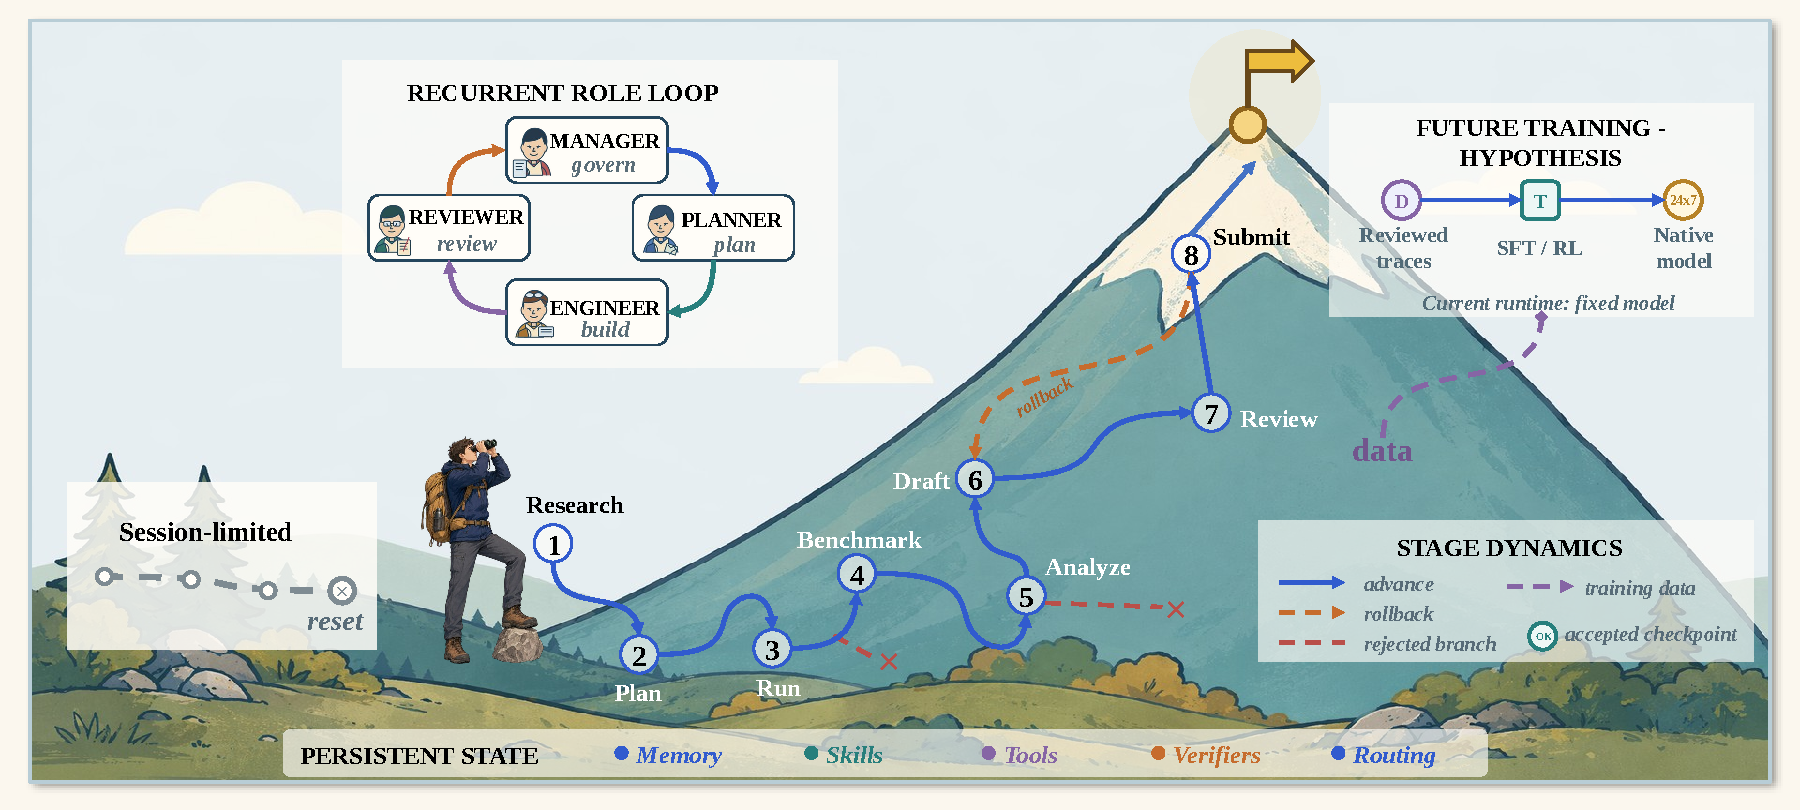
\includegraphics[width=0.95\linewidth]{figures/horizon_mountain.pdf}
  \caption{Operational model of long-horizon runtime self-evolution. The left card
  shows a session-limited route ending in reset. The central recurrent role loop is
  reused across eight Manager-controlled research Stages, while the blue route,
  orange rollback, and red rejected branches show that progress need not be
  monotone. Reviewed memory, Skills, tools, verifiers, and routing persist across
  missions. The purple path to future supervised fine-tuning and reinforcement
  learning (SFT/RL) is a research hypothesis; the current
  runtime changes persistent state while keeping model parameters fixed. Geometry
  is conceptual rather than an empirical scale.}
  \label{fig:horizon-mountain}
\end{figure}

\subsection{Role-State and Stage Dynamics}

The roles are not four sequential stations that execute once. Within a stage, the
campaign repeatedly applies the transition relation

\begin{equation}
  M \rightarrow P \rightarrow E \rightleftarrows R \rightarrow M,
  \label{eq:role-state-machine}
\end{equation}

where $M$, $P$, $E$, and $R$ denote Manager, Planner, Engineer, and Reviewer.
Reviewer continuation returns work to Engineer; an accepted or blocked verdict
returns control to Manager; and a Manager hold or rollback reopens planning. The
relation is an explanatory state-machine model of the implemented control flow, not
a claim that every transition must invoke a fresh model session.

Let $g_n$ be the current stage after the $n$th Manager decision. Legal transitions
are

\begin{equation}
  g_{n+1}
  \in \{g_n,\operatorname{next}(g_n)\}
  \cup \operatorname{prev}(g_n),
  \label{eq:stage-transition}
\end{equation}

corresponding to hold, advance to the immediate next stage, or rollback to an
earlier stage. For the research vertical, the ordered stages are research, plan,
benchmark, run, analysis, draft, review, and submission. Stage index and task-native
quality need not improve on every cycle: experiments can fail, review can reject a
branch, and later measurements can invalidate earlier assumptions. The intended ascent
is progress in the accepted frontier over many cycles, not monotonic improvement at
each transition.

\subsection{Dense-Intelligence Density}

The website expresses useful intelligence per unit wall-clock time as

\begin{equation}
  \rho_I(T)
  =\frac{1}{T}\int_0^T
  \dot N_{\mathrm{tok}}(t)\,
  \eta_r(t)\,\eta_a(t)\,\eta_v(t)\,dt.
  \label{eq:dense-density}
\end{equation}

$\dot N_{\mathrm{tok}}(t)$ is the instantaneous rate of token-mediated reasoning
and action. The factors $\eta_r(t)$, $\eta_a(t)$, and $\eta_v(t)$ represent the
fractions converted into relevant reasoning, effective action, and valid
verification. The product is intentionally stricter than token throughput: a run
that repeatedly reads the same state, emits activity without changing an artifact,
or accepts unchecked claims can consume many tokens while contributing little to
$\rho_I$.

\paragraph{Operational efficiency factors.}
The three factors describe how work is distributed within an analysis window. For
$W$, let $\mathcal{U}_k(W)$ be the attributable units for
$k\in\{r,a,v\}$: observable reasoning segments, executed actions, or verification
segments. We define
\begin{equation}
  \eta_k(W)
  =\frac{\sum_{u\in\mathcal{U}_k(W)} w(u)q_k(u)}
         {\sum_{u\in\mathcal{U}_k(W)} w(u)},
  \qquad 0\leq q_k(u)\leq1,
  \label{eq:operational-efficiency}
\end{equation}
where $w(u)$ is the attributable Token count for reasoning and verification, and
either one action or its measured cost for action efficiency. The attribution label
$q_k(u)$ records conversion into the intended function:

\begin{itemize}
  \item \textbf{Reasoning efficiency $\eta_r$.} A direct unit derives, revises, or
    rules out a named claim, lemma, blocker, or decision. Repeated context,
    narrative transitions, and notation-only rewriting are transition cost.
  \item \textbf{Action efficiency $\eta_a$.} A direct action changes an artifact,
    result set, accepted decision, or explored branch. A falsification action is
    productive when it certifies a dead branch; retries and interrupted no-op work
    are tracked separately. State synchronization and packaging form the auxiliary
    action category.
  \item \textbf{Verification efficiency $\eta_v$.} A direct verification unit
    compares a named claim with an explicit criterion or artifact, reruns an
    independent check, identifies a concrete defect, or issues a scoped verdict.
    Schema repair, reformatting, and checkpoint canonicalization enable review but
    belong to verification overhead rather than direct checking.
\end{itemize}

We report a direct-work value and an inclusive value that also counts successful
coordination and state maintenance. Equation~\ref{eq:dense-density} uses the three
factors as a multiplicative bottleneck model. Section~\ref{sec:vertical-trace}
measures them in the mathematical campaign, and
Appendix~\ref{app:formula-instantiation} gives the full calculation.

\subsection{Online Life and Runtime Evolution}

The second website object separates model parameters from the operating state
around the model:

\begin{equation}
  \begin{aligned}
    H_{t+1} &= U(H_t,\tau_t,E_t,K_{t+1}), \\
    \theta_{t+1} &= \theta_t.
  \end{aligned}
  \label{eq:runtime-update}
\end{equation}

with the public state definition

\begin{equation}
  H_t=\left\{\text{Memory},\text{Skills},\text{Tools},
  \text{Verifiers},\text{Routing}\right\}.
  \label{eq:website-state}
\end{equation}

$E_t$ is the subset of results admitted from mission $t$. The equality for
$\theta$ is a scope condition: online evolution does not require a gradient update
to the underlying model. Section~\ref{sec:method} refines $H_t$ into named ownership
surfaces, including task/evaluation definitions $Q_t$; subsequent updates treat
$Q_t$ as a component of $H_t$.
The contract argument records the admitted report-level projection. The update $U$
is partial; many missions change only memory, and some change no reusable component.

\subsection{Capability-Set Expansion}

Let $C_t$ denote the effective capability set available at time $t$. The website
writes verification-gated admission and the desired breadth/depth behavior as

\begin{equation}
  \begin{aligned}
    C_{t+1}
      &= C_t\cup\{c:\operatorname{Verify}(c,E_t)\geq\epsilon\}, \\
    W_{t+1} &\geq W_t,
    & D_{t+1}(d) &\geq D_t(d).
  \end{aligned}
  \label{eq:ood-expansion}
\end{equation}

where $W_t$ is frontier width across domains and $D_t(d)$ is depth within domain
$d$. The inequalities define retention desiderata over validated capability.
Skills can become stale, verifiers can be revised, and performance can regress on
harder instances. A negative result can still add value by excluding a failed branch even when the
effective capability set does not grow.

\subsection{Research Value}

Dense activity matters only when it produces new, valid, reusable information. The
website therefore defines the accumulated research value over horizon $T$ as

\begin{equation}
  V_R(T)
  =\int_0^T
  \rho_I(t)\,\Delta I(t)\,p_{\mathrm{valid}}(t)\,
  \eta_{\mathrm{reuse}}(t)\,dt,
  \label{eq:research-value}
\end{equation}

where $\Delta I(t)$ is information gain, $p_{\mathrm{valid}}(t)$ is the probability
that the claimed increment survives review, and
$\eta_{\mathrm{reuse}}(t)$ is the fraction that remains useful for later work.
Equation~\ref{eq:research-value} separates Token volume from the properties that
make a result useful: information gain, validity, and reuse. The experiments measure
these components in their native task units.

\subsection{The Information Advantage of Process Data}

Finally, the public formalization distinguishes the accepted artifact from the
trajectory that produced it:

\begin{equation}
  D_{\mathrm{process}}
  =\{(s_k,a_k,e_k,r_k,\Delta H_k)\}_{k=1}^{N}
  \supsetneq
  D_{\mathrm{final}}=\{y^\star\}.
  \label{eq:process-data}
\end{equation}

The process record contains states, actions, measurements, review feedback, and
runtime-state changes, including failed branches omitted from $y^\star$. This
additional information can reduce repeated search, guide later analysis, and provide
grounded material for later skill construction or evaluation. \systemname retains
typed, privacy-preserving observations and verdicts rather than private
chain-of-thought transcripts.

The set inclusion in Equation~\ref{eq:process-data} can be strengthened into a
decision-theoretic statement. Let $P$ denote a typed process record and let
$Y=g(P)$ be its final-artifact projection. For a downstream task $q$ with target
$Z_q$, loss $\ell_q$, and decision policy $\pi$, define the minimum achievable risk

\begin{equation}
  \mathcal{R}_q(X)
  =\inf_{\pi}\mathbb{E}\!\left[\ell_q\!\left(\pi(X),Z_q\right)\right].
  \label{eq:downstream-risk}
\end{equation}

\begin{paperbox}{Proposition 1: process-data dominance}
If $Y=g(P)$, then $\mathcal{R}_q(P)\leq\mathcal{R}_q(Y)$ for every downstream
decision problem $q$. The inequality is strict for some $q$ whenever two process
records can yield the same final artifact while implying different optimal next
actions. The proof is immediate: every policy using $Y$ can be reproduced from
$P$ by first applying $g$, while the reverse simulation need not exist. This is the
Blackwell-information ordering specialized to a research trajectory
~\citep{blackwell1953equivalent}.
\end{paperbox}

Dominance is informational, not computational. A raw trajectory can be too large,
stale, or contradictory to use efficiently. For a context budget $b$, the relevant
object is therefore a typed compression $\psi(P)$ that trades downstream risk
against retrieval and validation cost:

\begin{equation}
  \psi_b^\star
  =\arg\min_{\psi:\,\operatorname{size}(\psi(P))\leq b}
  \mathbb{E}_{q\sim\mathcal{D}}
  \left[\mathcal{R}_q(\psi(P))+\lambda_c C_{\mathrm{read}}(\psi(P))\right].
  \label{eq:process-compression}
\end{equation}

Equation~\ref{eq:process-compression} explains why an append-only event tape and a
bounded reviewed checkpoint serve different purposes. The tape preserves the more
informative experiment; the checkpoint approximates a decision-useful compression
under a finite context budget. Failed branches belong in the compression when they
change the next optimal action, not merely because they occurred.

\subsection{Reusable State and Compounding Intelligence}

Process data compounds only when an admitted state update improves later work. Let
$H_t\oplus\Delta H_t$ denote the state after accepting mission $t$, and let
$q_{t+1:t+L}$ be the next $L$ tasks. We define the discounted reuse value

\begin{equation}
  G_L(\Delta H_t)
  =\sum_{j=1}^{L}\gamma^{j-1}
  \left[
    \mathcal{R}_{q_{t+j}}(H_t)
    -\mathcal{R}_{q_{t+j}}(H_t\oplus\Delta H_t)
  \right].
  \label{eq:reuse-gain}
\end{equation}

$G_L>0$ means that the accepted memory, skill, verifier, routing rule, or certified
dead branch reduces future loss under a prespecified task distribution. $G_L<0$
captures negative transfer. This definition turns ``compounding intelligence''
from monotone rhetoric into a counterfactual claim: reuse must outperform a frozen
state on matched future tasks. Workflow-memory experiments show that induced
reusable routines can improve success and reduce steps
~\citep{wang2024workflowmemory}. Section~\ref{sec:discussion} connects this quantity
to the current \systemname traces.

The website's density and research-value equations can then be joined into a
protocol-specific \emph{verified reusable yield}:

\begin{equation}
  \mathcal{Y}_{\mathrm{PRI}}(W)
  =\frac{
    \sum_{t\in W}p_{\mathrm{valid},t}
    \left[\Delta I_t+\lambda_g G_L(\Delta H_t)\right]
  }{
    \sum_{t\in W}N_{\mathrm{tok},t}
  }.
  \label{eq:verified-reusable-yield}
\end{equation}

$\Delta I_t$ is immediate task-native information gain, such as a score
improvement, theorem strengthening, or certified branch elimination;
$p_{\mathrm{valid},t}$ is estimated by an external evaluator or a calibrated review
procedure; and $G_L$ measures future reuse. $\lambda_g$ converts immediate and
future value into one protocol-specific unit. Equation~\ref{eq:verified-reusable-yield}
connects immediate research output to future reuse. The current substitutions are
reported in Appendix~\ref{app:formula-instantiation}.

\subsection{Review as Selective Error Correction}

Let $C$ denote whether a proposed state increment is correct, $A$ whether the
Reviewer accepts it, $p=\Pr(C=1)$ the proposal base rate,
$\alpha=\Pr(A=1\mid C=1)$ Reviewer sensitivity, and
$\beta=\Pr(A=1\mid C=0)$ false-acceptance rate. Bayes' rule gives

\begin{equation}
  \Pr(C=1\mid A=1)
  =\frac{\alpha p}{\alpha p+\beta(1-p)}.
  \label{eq:review-precision}
\end{equation}

If $\alpha>\beta$, accepted state is more precise than the proposal stream; review
acts as a selective error-correction channel. Its operating point balances accepted
precision, recall, and Token cost. Section~\ref{sec:results} reports the observed
repair and recovery rates.

\subsection{Role-Resolved Vertical Traces}

Endpoint metrics do not show how an Agent system actually conducts research. We
therefore project each mission trajectory in Equation~\ref{eq:trajectory} onto
the four role-owned actions

\begin{equation}
  \phi(\tau_t)=\left(m_t,p_t,x_t,r_t,\Delta H_t\right),
  \label{eq:role-resolved-trace}
\end{equation}

where $m_t$ is the Manager's objective or stage decision, $p_t$ is the Planner's
bounded task and dependency decision, $x_t$ is the Engineer's artifact-producing
execution, $r_t$ is the structured completion decision together with its source,
and $\Delta H_t$ is the durable state update exposed to later missions. The
decomposition makes two authority constraints explicit: only the Manager changes
campaign stage, while mission completion records either an allowed Engineer
self-review or a required/requested independent Reviewer verdict. Vertical policy
and stage-closing tasks prevent Engineer self-certification where independent
review is mandatory; the Planner may propose future work but cannot certify the
mission.

A vertical trace is useful when these tuples remain linked across many missions.
It shows whether the objective survived failures, whether the Planner consumed
previously accepted state, whether the Engineer changed real artifacts, whether
the Reviewer rejected or redirected incomplete work, and which decisions became
inputs to the next mission. This explanatory model organizes the Agent workflow;
Section~\ref{sec:vertical-trace} applies it to one mathematical campaign.
